\subsection{Hall Sensor}
There are two hall sensors implemented on the vehicle, one on each belt, at the front gear (See \figref{vehicleDescriptionDriveTrain} in \secref{sec:Vehicledescription}). There are two hall sensors to measure the speed, because the belts run at different speeds when the vehicle is turning. The sensors are placed beside the front gears, on which there are four magnets, placed so that there is a quarter of a turn between them. The hall sensor is illustrated on \figref{HallSensor}.

 \begin{figure}[H]
	\centering
	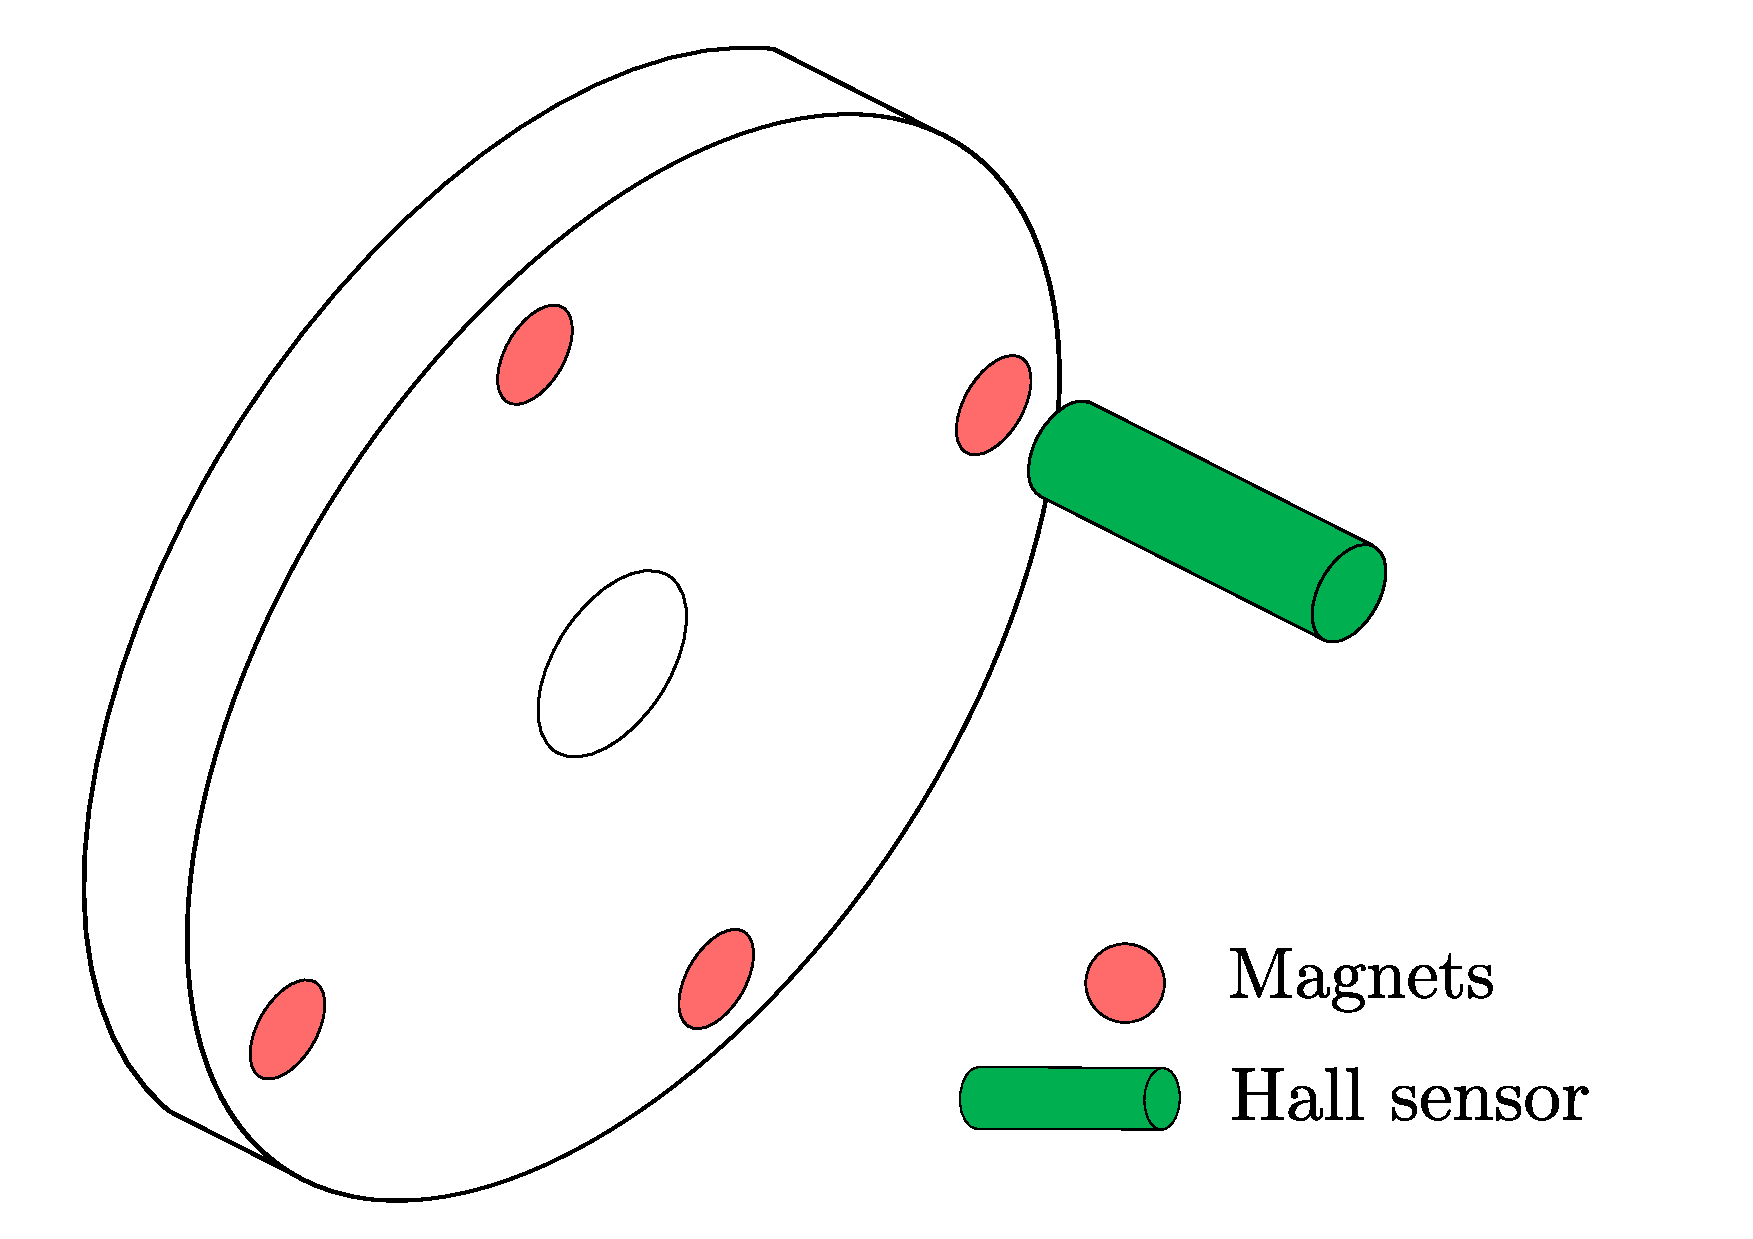
\includegraphics[scale=0.4]{figures/HallSensor3D.pdf}
	\caption{Illustration of the front gear, with the magnets and the hall sensor. The hall sensor is placed stationary beside the rotating gear.}
	\label{HallSensor}
\end{figure}

A hall sensor is a sensor that is activated when exposed to a magnetic field. This gives a voltage output each time one of the magnets is in front of the hall sensor. Because of this, there is a signal each quarter of a turn of the gear. As the distance between each magnets is not exactly a quarter of a turn, the distance between the magnets is not the same. The calculations will be taken for each magnets independently, because of this difference.
By measuring the time between five outputs, as the first and the fifth output is from the same magnet, the time of a whole rotation of the gear can be found. By knowing the distance the vehicle travels for a full rotation of the gear, the speed can be calculated.

When the vehicle is starting to move, the speed of the first turn of the gear can not be calculated. This is because two signal from the same magnet are needed before the speed can be calculated. So the first four output from the hall sensor will be saved and at the fifth output, after a whole turn, the speed related to the first magnet will be calculated.\\

The hall sensors are used to measure the speed of the two belts, which will run at different speeds when the vehicle is turning. Now that the components linked to the velocity  are described, the steering material will be analysed.
